\documentclass[10pt,letterpaper]{article}
\usepackage[margin=.85in]{geometry}
\usepackage[T1]{fontenc}\usepackage{lmodern,graphicx,booktabs,amsmath,xcolor,hyperref,xurl,caption,fancyhdr}
\hypersetup{colorlinks=true,urlcolor=teal,linkcolor=teal,pdftitle={Budget a buffer for day-ahead wind shortfalls},pdfauthor={James Jean}}
\pagestyle{fancy}\fancyhf{}\fancyhead[L]{\small Wind shortfall buffer / Study 26}\fancyhead[R]{\small Independent retrospective study}\fancyfoot[C]{\thepage}
\setlength{\headheight}{14pt}\setlength{\parindent}{0pt}\setlength{\parskip}{6pt}\captionsetup{font=small,labelfont=bf,hypcap=false}
\begin{document}
{\small\color{teal} WIND FORECAST REVIEW / EXPLICIT SHORTFALL ASSUMPTIONS\par}
\vspace{7pt}{\LARGE\bfseries Budget a buffer for day-ahead wind shortfalls\par}
\vspace{6pt}James Jean \hfill 30 October 2026
\section*{The decision}
A planner booking a buffer against a wind forecast has to balance unused capacity against uncovered shortfall. Average forecast error alone does not answer that question. This study compares six simple rules using historical Elia onshore wind forecasts and reported production, with explicit hypothetical capacity caps and relative shortfall penalties.

\textbf{Finding.} Under the primary assumption that uncovered shortfall costs five times as much as a booked buffer, the development-selected Q75 rule lowers mean proxy cost from \textbf{117.120 to 87.820} in Flanders and \textbf{103.987 to 75.474} in Wallonia. Each region has 26,260 eligible held hours. These are weighted MW proxy quantities, \emph{not currency or measured savings}. Observed no-uncovered-shortfall coverage is \textbf{79.954\% and 75.091\%}, respectively.

\textbf{What changes the decision.} At a penalty ratio of two, the same Q75 buffer costs more than zero in both regions. Q80 has a slightly lower primary held cost than Q75 in Wallonia; the frozen development choice is retained. The fixed mean-bias correction also worsens held point-forecast MAE in both regions. A useful buffer under one assumed loss is a different claim from a better forecast or improved grid reliability.

\begin{center}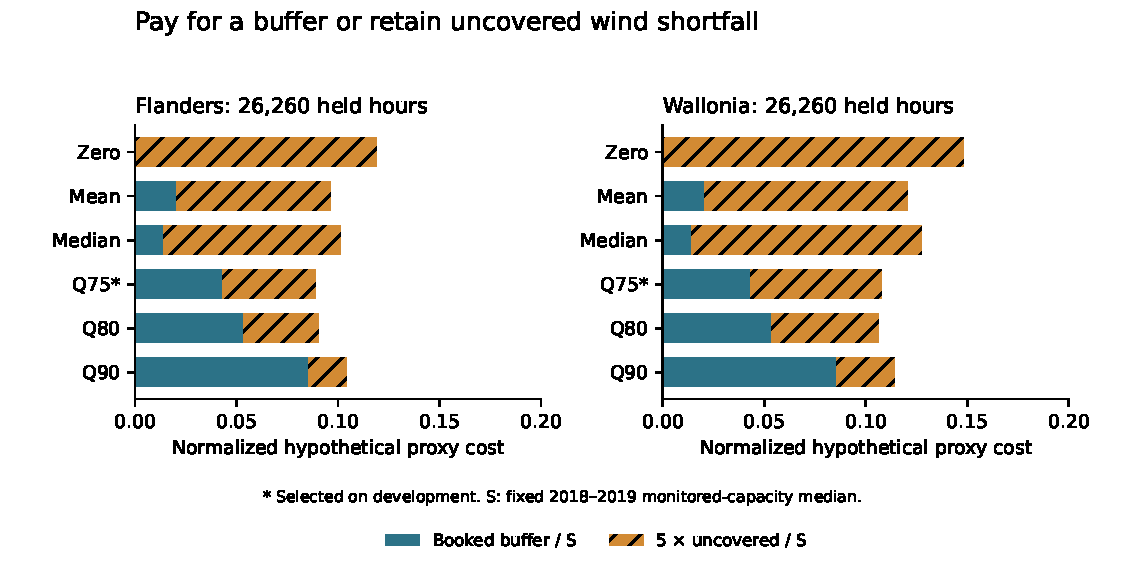
\includegraphics[width=\linewidth]{images/cost_components.pdf}\end{center}
\captionof{figure}{Primary scenario: penalty ratio five and cap ten percent of an earlier monitored-capacity reference $S$. Bars show booked buffer and weighted uncovered shortfall, normalized by $S$. Q75 is selected on development data; all six candidates remain visible.}

\textbf{Practical recommendation.} State the cost of uncovered shortfall and feasible buffer capacity before choosing a rule. Preserve a zero-buffer comparison and check whether the policy transfers. No physical dispatch, market cost, actual reserve requirement, financial saving or reliability gain was measured. Reported upscaled generation is not independently validated meter truth.
\newpage
\section*{1. Source, calendar and measurement limits}
Elia Transmission Belgium SA's historical wind dataset ods031 [1] provides reported measured-and-upscaled generation, source-labeled day-ahead 6 PM forecasts, monitored capacity and category keys. Values are running-average MW for fifteen-minute intervals; download timestamps identify interval starts in UTC. The historical proposal named EIA930, whose official elements provide demand forecasts rather than renewable generation forecasts [2]. Elia fits the renewable-shortfall question without treating demand as wind.

The fixed cohort contains onshore, DSO-connected Flanders and Wallonia during 2018--2023. Official metadata warns about offshore measured/upscaled discrepancies during those years; offshore was excluded before collection. This does not establish that the retained onshore estimates are fully validated. Upscaling, source revisions and curtailment can affect comparisons. An empty published curtailment indicator does not establish the absence of owner-requested reductions.

Each region/year was captured once as CSV and JSON after protocol revision \texttt{8769aa0}. Exact requests, UTC start/end times, HTTP status, relevant response headers, bytes and hashes were saved before parsing. Dataset processing markers matched before and after the batch. Independent Pandas/JSON parsing reconciled all 420,672 selected records as complete multisets and checked public source-row bindings. The public subset contains nine factual fields plus provenance identifiers; originals and source documents remain privately retained.

\begin{center}\begin{tabular}{rrrr}\toprule
Year & Planned hours per region & Eligible Flanders & Eligible Wallonia\\\midrule
2018 & 8760 & 8760 & 8760 \\
2019 & 8760 & 8760 & 8760 \\
2020 & 8784 & 8784 & 8784 \\
2021 & 8760 & 8756 & 8756 \\
2022 & 8760 & 8760 & 8760 \\
2023 & 8760 & 8744 & 8744 \\
\bottomrule\end{tabular}\end{center}
\textbf{Table 1.} Full UTC calendar. Each hour requires four distinct eligible quarter-hours. Eight quarter-hour slots lack measured values and 152 lack monitored capacity, leaving 105,128 of 105,168 planned region-hours eligible. Forty hours remain unavailable; none is interpolated or filled with zero. Every region/year/quarter passes the predeclared ninety-percent hourly-coverage gate. That is a completeness check, not a meter-quality certificate.

The source screen requires aligned timestamps, the intended categories and PT15M resolution, finite nonnegative forecast/measurement values and positive finite capacity. Duplicate keys would be excluded in full. The full source-row and planned-slot ledgers remain available. No forecast-error threshold, favorable-outcome screen or curtailment deletion is applied. Hourly MW is the arithmetic mean of four quarter-hour MW values, not their sum. Multiplication by one hour gives an energy-equivalent quantity; it does not establish actual reserve deployment.

The source license page applies CC BY 4.0 [3,4]. Attribution, source/license links, change notice and no-endorsement language accompany the minimal projection. The source's general disclaimer redirect returned 403; no bypass was attempted. The accessible specific license and schema control this data use. Current source-labeled historical forecasts do not supply an original per-record issuance receipt or every revision. This is a retrospective evaluation, not an exact-vintage live simulation.
\newpage
\section*{2. Rules, assumptions and a protected selection}
Let $e=f-y$ be forecast minus reported generation in MW. Positive $e$ represents a wind shortfall relative to forecast. Flanders 2018--2019 contributes 17,520 eligible training error labels. Define fixed regional scale $S$ as the median earlier monitored capacity: \textbf{985.430 MW} for Flanders and \textbf{701.610 MW} for Wallonia. Only Wallonia's earlier capacity covariates are used; its error labels do not fit or select a policy. This is a geographic outcome holdout with capacity adaptation, not a completely unseen-domain claim.

Fit six statistics $b$ to signed normalized Flanders errors $e/S$: zero, arithmetic mean, ordinary midpoint median, and nearest-rank quantiles Q75, Q80 and Q90. The quantile uses ordered value $x_{\lceil qn\rceil}$, with one-based rank. Negative residuals remain negative during fitting. These are established fixed estimators; there is no ML training, search extension or random seed.

For a declared cap ratio $c$, book $r=S\min(c,\max(0,b))$. Uncovered shortfall is $u=\max(f-y-r,0)$ and excess buffer is $\max(r-\max(f-y,0),0)$. A covered hour has $f-y\leq r$, including exact equality. The assumed loss is
\[ L=r+\lambda u,\qquad c\in\{0.05,0.10,0.20\},\quad\lambda\in\{2,5,10\}. \]
Primary selection uses $c=0.10$ and $\lambda=5$. The cap is a scenario fraction of an earlier capacity reference, not observed available reserve. The penalty is a relative assumption, not an electricity price or reliability valuation. Downward balancing, ramps, dispatch constraints and storage duration are outside this one-sided proxy.

Flanders 2020 supplies 8,784 development hours in four fixed calendar-quarter blocks. Choose the lowest equal-quarter mean $L/S$; exact ties prefer the lower candidate index. All six candidates remain below. A quarter mean is computed on its eligible hours before the four blocks receive equal weight.

\begin{center}\begin{tabular}{lrr}\toprule
Rule & Fitted normalized statistic $b$ & Development objective\\\midrule
Zero & 0.000000 & 0.113521 \\
Mean & 0.020413 & 0.090186 \\
Median & 0.014051 & 0.095042 \\
Q75 (selected) & 0.043197 & 0.085166 \\
Q80 & 0.053545 & 0.087691 \\
Q90 & 0.085359 & 0.104278 \\
\bottomrule\end{tabular}\end{center}
\textbf{Table 2.} Fixed finite candidate set and primary development objective. Q75 is selected. Negative or capped statistics would still remain in the export; fitting is not done on positive errors alone.

Without the cap, minimizing expected $r+\lambda(e-r)_+$ leads, under suitable conditions, to the $1-1/\lambda$ error quantile. This motivates Q80 when $\lambda=5$; it does not guarantee its development or held superiority. Matching a forecast functional to its loss is an established principle [5], not a novelty claim here.

Twenty-nine dependency hashes were committed and pushed in freeze revision \texttt{ad928f1} before any held policy or point summaries. They bind source, calendar, fitting/selection code, independent checkers, fixtures and development exports. Held years 2021--2023 do not change the selected policy, objective, scenarios or reporting blocks.
\newpage
\section*{3. Held costs and point accuracy are different results}
\begin{center}\scriptsize\begin{tabular}{llrrrr}\toprule
Region & Rule & Buffer MW & Uncovered MW & Proxy cost & Coverage (\%)\\\midrule
Flanders & Zero & 0.000 & 23.424 & 117.120 & 47.704 \\
 & Mean & 20.115 & 14.952 & 94.878 & 66.542 \\
 & Median & 13.846 & 17.206 & 99.874 & 61.478 \\
 & Q75 (selected) & 42.568 & 9.051 & 87.820 & 79.954 \\
 & Q80 & 52.765 & 7.230 & 88.913 & 84.204 \\
 & Q90 & 84.115 & 3.746 & 102.845 & 92.510 \\
Wallonia & Zero & 0.000 & 20.797 & 103.987 & 43.222 \\
 & Mean & 14.322 & 14.057 & 84.609 & 61.337 \\
 & Median & 9.858 & 15.892 & 89.319 & 56.474 \\
 & Q75 (selected) & 30.307 & 9.033 & 75.474 & 75.091 \\
 & Q80 & 37.568 & 7.389 & 74.514 & 79.623 \\
 & Q90 & 59.889 & 4.062 & 80.199 & 89.383 \\
\bottomrule\end{tabular}\end{center}
\textbf{Table 3.} Primary held scenario on 26,260 eligible hours per region. Mean proxy cost is buffer plus five times uncovered MW. Its units are weighted MW, not currency. All six rules use the same hours and target values. Coverage is the observed fraction with no uncovered shortfall, not a confidence guarantee or a calibrated quantile probability.

Q75 has the lowest primary held proxy cost among these six candidates in Flanders. Q80 is slightly lower in Wallonia; Q75 remains the protected development choice. Larger Q90 buffers increase coverage but also increase the primary cost relative to Q75. That tradeoff is visible rather than hidden behind a single coverage number. No actual reserve fleet was dispatched, and the source's scale $S$ is not a reliability target.

Three fixed point-forecast comparators are reported separately: source unchanged, subtract the earlier mean signed normalized error times regional $S$, or subtract its median times $S$. Corrected forecasts are clipped at zero. They are not chosen on held results and are not the buffer-policy selection criterion.

\begin{center}\scriptsize\begin{tabular}{llrrr}\toprule
Region & Point forecast & MAE (MW) & RMSE (MW) & Signed bias (MW)\\\midrule
Flanders & Source & 49.296 & 71.003 & -2.448 \\
 & Mean corrected & 51.814 & 74.304 & -21.909 \\
 & Median corrected & 50.414 & 72.752 & -16.003 \\
Wallonia & Source & 38.026 & 54.776 & 3.568 \\
 & Mean corrected & 38.497 & 55.629 & -10.382 \\
 & Median corrected & 37.929 & 54.997 & -6.144 \\
\bottomrule\end{tabular}\end{center}
\textbf{Table 4.} Same held hours. MSE and scale-normalized MAE remain in the complete exports. The fixed mean correction worsens MAE and RMSE in both regions. Median correction slightly improves Wallonia MAE while worsening its RMSE; both corrections worsen Flanders MAE. A favorable buffer result does not turn these mixed point-forecast results into an accuracy improvement.

Earlier signed-error behavior need not persist. A correction estimated in 2018--2019 can over-adjust later forecasts. This retrospective comparison describes that failure; it does not identify a causal reason for the underlying source forecast changes or validate a new forecast service. No held-based refit or selective removal of unfavorable hours is performed.
\newpage
\section*{4. Geographic transfer and time variation}
The same normalized Q75 statistic is transferred to Wallonia using its earlier monitored-capacity scale. This yields a different MW action but no use of Wallonia error labels in fitting or selection. Lower observed coverage there shows why geographic transfer needs direct evaluation.

\begin{center}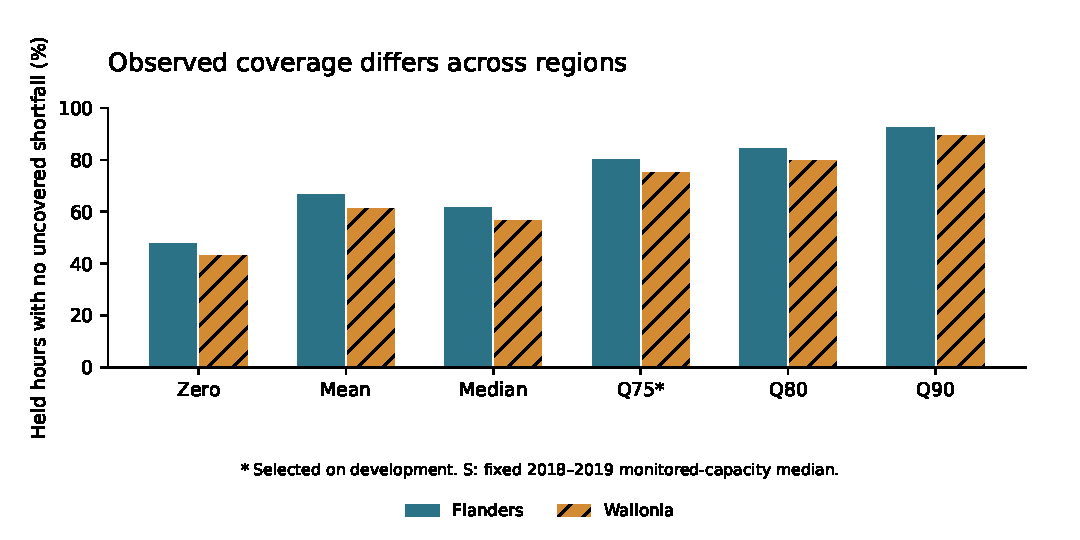
\includegraphics[width=.98\linewidth]{images/observed_coverage.pdf}\end{center}
\captionof{figure}{Observed held-hour coverage in the primary scenario. Both axes and the zero-buffer baseline remain visible. Q75 is the frozen development choice, not a promise of seventy-five-percent or any other population coverage. Reported production and source-vintage qualifications still apply.}

\begin{center}\small\begin{tabular}{llrrrr}\toprule
Region & Year & Eligible hours & Zero cost/$S$ & Q75 cost/$S$ & Q80 cost/$S$\\\midrule
Flanders & 2021 & 8756 & 0.1110 & 0.0806 & 0.0821 \\
 & 2022 & 8760 & 0.0863 & 0.0711 & 0.0752 \\
 & 2023 & 8744 & 0.1593 & 0.1157 & 0.1134 \\
Wallonia & 2021 & 8756 & 0.1243 & 0.0896 & 0.0897 \\
 & 2022 & 8760 & 0.1236 & 0.0919 & 0.0926 \\
 & 2023 & 8744 & 0.1968 & 0.1413 & 0.1363 \\
\bottomrule\end{tabular}\end{center}
\textbf{Table 5.} Primary annual normalized proxy cost. All fixed calendar-quarter results are also exported, including incomplete hours in the denominator ledger. The held comparison uses common eligible hours across rules; missing hours are not successful covered outcomes.

Only two regional aggregates and three held years are observed. Hours are serially dependent and are not independent experiments. There is no randomized policy deployment, probability sample or universal confidence interval. Descriptive paired losses for this finite cohort support the comparisons shown; they do not establish a causal reliability or financial benefit. Transfer to another region, technology or dispatch setting needs its own source and decision-loss evidence.
\newpage
\section*{5. Cost assumptions can reverse the decision}
\begin{center}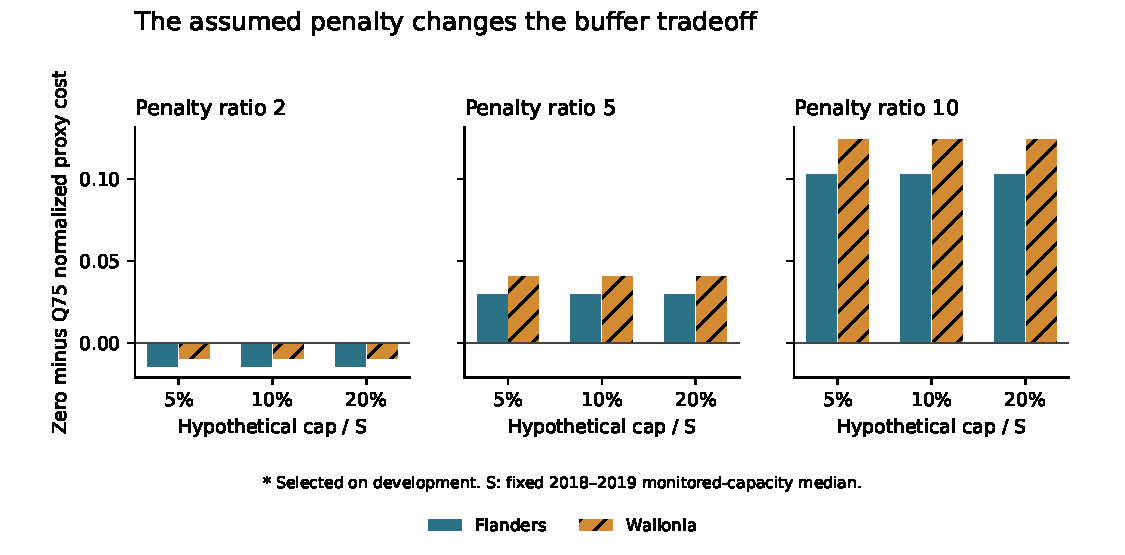
\includegraphics[width=.98\linewidth]{images/scenario_sensitivity.pdf}\end{center}
\captionof{figure}{Zero minus selected-Q75 normalized proxy cost. Positive values favor the buffer under the declared loss; negative values favor zero. The uncovered-shortfall penalty changes that ordering. These are scenario comparisons, not measured savings or a fitted cost model.}

\begin{center}\begin{tabular}{rrrr}\toprule
Penalty ratio & Cap/$S$ & Flanders difference & Wallonia difference\\\midrule
2 & 5\% & -0.0140 & -0.0097 \\
2 & 10\% & -0.0140 & -0.0097 \\
2 & 20\% & -0.0140 & -0.0097 \\
5 & 5\% & 0.0297 & 0.0406 \\
5 & 10\% & 0.0297 & 0.0406 \\
5 & 20\% & 0.0297 & 0.0406 \\
10 & 5\% & 0.1027 & 0.1245 \\
10 & 10\% & 0.1027 & 0.1245 \\
10 & 20\% & 0.1027 & 0.1245 \\
\bottomrule\end{tabular}\end{center}
\textbf{Table 6.} Paired mean-loss differences for the same held hours. Q75 is retained across all scenarios. Every candidate's full nine-scenario result remains in the machine-readable export; the selected-only table does not replace those comparisons.

At penalty ratio two, the booked Q75 buffer is more costly than zero in both regions. At ratios five and ten, it has lower proxy cost. The selected normalized statistic lies below the smallest five-percent cap, so its action is unchanged across these three caps. Flat selected-policy sensitivity does not establish that capacity never matters: other candidates can bind at the smallest cap, and a real system's feasible capacity is unmeasured here.

\textbf{Use in a review.} Ask the decision owner to specify a justified shortfall penalty and feasible buffer capacity. Compare zero, the protected rule and simpler alternatives on the same hours. Check point-forecast accuracy separately, retain adverse scenarios and evaluate another region before claiming transfer. A reserve or storage decision additionally needs ramp, duration, network, market and operational constraints that this study does not model.
\newpage
\section*{6. Reproduction and next use}
Independent source reconciliation performed 7,992,809 field and structural comparisons on the captured CSV/JSON projections and bindings. A separate SQLite full-calendar join and eighty-digit Decimal integration checked every source row, planned slot and hour in 6,099,749 comparisons. Independent result reconstruction uses separate SQL role selection, signed Decimal training inputs and exact-rational policy/point arithmetic, with 2,271,889 development and 13,586,122 held comparisons. Finite comparison counts are not a universal correctness or accuracy estimate.

Thirty invented fixtures cover full-hour integration, missing and duplicate slots, UTC rollover, finite/sign rules, signed residuals, quantile ranks, median conventions, capacity clipping, exact event boundaries, surplus versus shortfall, nonnegative corrected forecasts, policy-scale transfer, exact ties and asymmetric-loss examples. They are excluded from empirical data and outcomes. Source labels, policy actions and hypothetical penalties remain explicitly distinguished.

Offline replay creates a temporary local Git clone, rebuilds inputs and all results, reruns independent checks and fixtures, and compares 21,916,240 CSV fields including headers plus eight JSON documents. Original files remain unchanged and no new source network is used. Original figure checks cover 54 source values, 432 actual SVG rectangle coordinates and nine artifact hashes. Paper displays are separately rebuilt from observation exports, then bounded PDF action/hash checks and actual rendered-page inspection are required. Exact-candidate and main Linux success, matching tested/merged content and a remote annotated tag are later release gates; local paper evidence does not assert those later gates passed.

\textbf{Run locally.} Use Python 3.12, install \texttt{requirements.txt} and run \texttt{python src/reproduce.py}. Figure, paper and canonical-Git checks are listed in the workflow. Full two-format reconciliation additionally requires the privately retained original exports. Compressed policy rows store actions and uncovered quantities once per cap: any declared penalty reconstructs loss as reserve plus penalty times uncovered. A penalty changes the score, not the already booked action.

\textbf{Next evidence.} Evaluate a new source vintage or genuinely independent region with a decision owner who can justify the actual constraints and losses. Validate production measurement and forecast issuance versions before an operational claim. The implementation uses established quantiles and asymmetric losses; no new estimator, exhaustive novelty, peer review, deployment or realized benefit is claimed. Formal-publication projects, including Azure optimization, remain excluded from this public independent program.

\section*{References}
{\footnotesize
[1] Elia Transmission Belgium SA. Wind power production estimation and forecast on Belgian grid (Historical), ods031. \url{https://opendata.elia.be/explore/dataset/ods031/information/}. Captured 30 October 2026; metadata, exact requests and hashes retained. Minimal projected fields, calendar flags, hourly averaging and hypothetical policy calculations are this study's changes; no endorsement is implied.\par
[2] U.S. Energy Information Administration. About EIA-930 data. \url{https://www.eia.gov/electricity/930-content/about.html}. Accessed 30 October 2026.\par
[3] Elia Open Data License. \url{https://opendata.elia.be/pages/licence/}. Public license HTML applies CC BY 4.0, subject to its stated law/jurisdiction provisions. Accessed 30 October 2026.\par
[4] Creative Commons. Attribution 4.0 International. \url{https://creativecommons.org/licenses/by/4.0/}. Attribution, license link and change notice retained; no endorsement claim.\par
[5] Gneiting, T. Making and Evaluating Point Forecasts. Primary author manuscript, arXiv:0912.0902, 2010 version. \url{https://arxiv.org/abs/0912.0902}. Established matching of scoring functions and forecast functionals; no priority claim here.}
\end{document}
